% Source: Unknown
% File: ".pdf"
% Access: Unknown

% comment out for student version
% \ifdefined\Student\relax\else\def\Teacher{}\fi

\documentclass[12pt]{article}

\title{Activity \#24: Pointers}
\author{Unknown}
\newcommand{\activityeditor}{Preston Carman}
\newcommand{\activitysource}{\url{}}
\date{Spring 2022}

\input{../../cspogil.sty}
\usepackage{tikz}

\begin{document}

  \begin{center}
    \maketitle
    \rolenames
  \end{center}
  
  \keyquestions{
    \item Model 1, Question \#6
    \item Model 2, Question \#10.b
    \item Model 2, Question \#12.c
  }

  \newpage
  \maketitle

  In this activity, you will work in teams of 3--4 students to learn new concepts.
  This activity will introduce you to pointers in C++.

  \guide{
    \item Define what pointers are and explain how they work.
    \item Explain how to use the reference and dereference operators.
  }{
    \item Write C++ code that utilizes pointers.\\[-5pt]
  }{
    No additional notes.
  }

  \model{A First Program with Pointers}
  \begin{center}
    \small
    \begin{tabular}{p{2.8in}p{0.1in}p{2.8in}}
      \begin{minipage}{2.8in}
        \begin{cpplst}
#include <iostream>

using namespace std;

int main() {
  int myArray[] = {40, 30, 20, 10};
  int *p = myArray;
  // Your code goes here
  cout << "Value of p: " << p << endl;
  cout << "Value of *p: " << *p << endl;
  cout << "Value of myArray: ";
  for (int i = 0; i < 3; i++) {
    cout << myArray[i] << ",";
  }
  cout << myArray[3] << endl;
}
        \end{cpplst}      
      \end{minipage}
      & &
      \begin{minipage}{2.8in}
        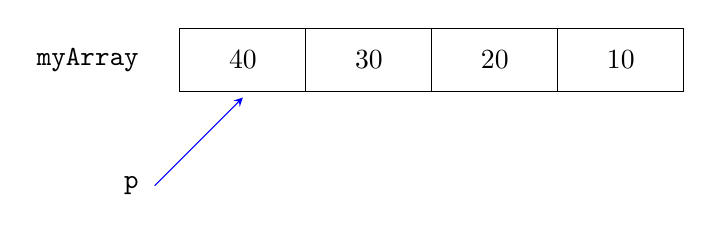
\begin{tikzpicture}[scale=0.8]
          \node[right] at (-0.5,0.5) [left] {\tt myArray};
          \draw (0,0) rectangle (8,1);
          \draw (2,0) -- (2,1);
          \draw (4,0) -- (4,1);
          \draw (6,0) -- (6,1);
          \node at (1,0.5) {$40$};
          \node at (3,0.5) {$30$};
          \node at (5,0.5) {$20$};
          \node at (7,0.5) {$10$};
          \node at (-0.5,-1.5) [left] {\tt p};
          \draw[blue,-stealth] (-0.4,-1.5) -- (1,-0.1);
        \end{tikzpicture}
      \end{minipage}
    \end{tabular}
  \end{center}
  
  {\it\large Refer to Model 1 above as your group develops consensus answers
    to the questions below.}

  \quest{30 min}
    
  \Q The file {\tt activity24a.cpp} contains this code.
    Run it and record the output on the lines below.
    \begin{enumerate}
      \itemsep 10pt
      \begin{multicols}{2}
        \item {\tt Value of p: } \hspace{0.5in} \ans[1.25in]{a memory location}
        \item {\tt Value of *p: } \hspace{0.4in} \ans[1.25in]{40}
        \item {\tt Value of myArray: } \hfill \ans[1.25in]{40, 30, 20, 10}
      \end{multicols}
    \end{enumerate}

  \vskip -15pt
    
  \Q Run the code several times.  Describe how (if at all) the
    output changes each time you run the program.
    \begin{answer}[0.5in]
      Yes, the output from line 9 changes each time it is run.
    \end{answer}

  \Q A {\it pointer} is a variable that holds a memory address,
    rather than data.  The diagram on the right of the model
    depicts the pointer relationship in this code.
    \begin{enumerate}
      \item Based on the diagram, which variable is a pointer?
        \begin{answer}[0.5in]
          {\tt p} is the pointer variable.
        \end{answer}

      \item Now looking at the code, how is a pointer declared in C++?
        \begin{answer}[0.75in]
          By placing an asterisk ({\tt *}) before the variable name
          in the declaration.
        \end{answer}

      \item How does this explain what you observed in question 2
        above?
        \begin{answer}[0.75in]
          Since {\tt p} is a pointer variable, its value is a memory
          address.  Memory addresses can change each time the program
          is run, which is why the output from line 10 changes.
        \end{answer}

      \item Does a pointer have a data type like other variables? Explain.      
        \begin{answer}[0.75in]
          Yes.  In this case, {\tt p} is declared as an {\tt int*},
          which means it is a pointer to an integer.  This means
          that the memory address stored in {\tt p} points to
          an integer value.
        \end{answer}
    \end{enumerate}

  \vskip -15pt
    
  \Q Now add each of the following code snippets in line 8, one at a time.
    Run the code and record its output.
    \begin{enumerate}
      \item \cpp{p++}
        \begin{enumerate}
          \itemsep 10pt
          \begin{multicols}{2}
            \item {\tt Value of p: } \hspace{0.2in} \ans[1.25in]{a memory location}
            \item {\tt Value of *p: } \hspace{0.1in} \ans[1.25in]{30}
            \item {\tt Value of myArray: } \hfill \ans[1.25in]{40, 30, 20, 10}
          \end{multicols}
        \end{enumerate}\par\vskip 10pt

      \item \cpp{(*p)++}
        \begin{enumerate}
          \itemsep 10pt
          \begin{multicols}{2}
            \item {\tt Value of p: } \hspace{0.2in}\ans[1.25in]{a memory location}
            \item {\tt Value of *p: } \hspace{0.1in} \ans[1.25in]{40}
            \item {\tt Value of myArray: } \hfill \ans[1.25in]{41, 30,2 0,10}
          \end{multicols}
        \end{enumerate}\par\vskip 10pt

      \item \cpp{*(p+2) += 2;}
        \par\vskip 10pt
        \begin{enumerate}
          \itemsep 10pt
          \begin{multicols}{2}
            \item {\tt Value of p: } \hspace{0.2in} \ans[1.25in]{a memory location}
            \item {\tt Value of *p: } \hspace{0.1in} \ans[1.25in]{40}
            \item {\tt Value of myArray: } \hfill \ans[1.25in]{40, 30, 22,10}
          \end{multicols}
        \end{enumerate}
    \end{enumerate}

  \newpage
    
  \Q Complete the diagram below to show the contents of
    {\tt myArray} and the pointer relationship between
    {\tt p} and {\tt myArray} after line 8 of the model 
    was changed as indicated above.
    \begin{enumerate}
      \begin{multicols}{2}
        \item \cpp{p++}\par\vskip 10pt
          \begin{minipage}{2.75in}
            \begin{tikzpicture}[scale=0.6]
              \node at (-0.5,0.5) [left] {\tt myArray};
              \draw (0,0) rectangle (8,1);
              \draw (2,0) -- (2,1);
              \draw (4,0) -- (4,1);
              \draw (6,0) -- (6,1);
              \node at (-0.5,-1.5) [left] {\tt p};
            \end{tikzpicture}
          \end{minipage}

        \item \cpp{(*p)++}\par\vskip 10pt
          \begin{minipage}{2.75in}
            \begin{tikzpicture}[scale=0.6]
              \node at (-0.5,0.5) [left] {\tt myArray};
              \draw (0,0) rectangle (8,1);
              \draw (2,0) -- (2,1);
              \draw (4,0) -- (4,1);
              \draw (6,0) -- (6,1);
              \node at (-0.5,-1.5) [left] {\tt p};
            \end{tikzpicture}
          \end{minipage}
      \end{multicols}
    \end{enumerate}

  \vskip -30pt
          
  \Q Write a single line of code referencing only {\tt p} 
    that does the following when added \key\\[-2.5mm] on line 8.
    \par\vskip 10pt
    \begin{enumerate}
      \itemsep 10pt
      \item Adds 5 to the first entry in {\tt myArray} (making it 45):
        \hfill\ans[2in]{\cpp{*p += 5}}

      \item Changes the second line of output to ``{\tt Value of *p: 10}'':
        \hfill\ans[2in]{\cpp{p+=3}}
        
      \item Adds 5 to the 2nd entry in {\tt myArray} (making it 35):
        \hfill\ans[2in]{\cpp{*(p+1) += 5}}          
    \end{enumerate}
    
  \Q Finally, place the command \cpp{p -= 10;} on line 8
    of the model and run the code several times.
    \begin{enumerate}
      \item What happens to the output each time you run the program?
        \begin{answer}[0.75in]
          The program crashes with a segmentation fault each time.
        \end{answer}

      \item This example illustrates one of the {\it dangers} of
        using pointers.  In your own words, describe what that danger is.
        \begin{answer}[1.25in]
          Answers will vary.
        \end{answer}
    \end{enumerate}

  \newpage
  \model{A Second Program with Pointers}
  \begin{center}
    \small
    \begin{minipage}{4.5in}
      \begin{cpplst}
#include <iostream>

using namespace std;

int main() {
  int numOne = 1892;
  int numTwo = 1973;
  int numThree = 2008;
  int *numArray[3] = {&numOne, &numTwo, &numThree};
  int *p;

  p = &numOne;
  cout << "Number: " << *p << endl;
  p = &numTwo;
  cout << "Number: " << *p << endl;
  p = &numThree;
  cout << "Number: " << *p << endl;
}
      \end{cpplst}
    \end{minipage}
  \end{center}
  
  {\it\large Refer to Model 2 above as your group develops consensus answers
    to the questions below.}

  \quest{20 min}
    
  \Q Without running any code, predict what the output of this
    program will be.
    \begin{answer}[0.75in]
      Number: 1892
      Number: 1973
      Number: 2008
    \end{answer}
    
  \Q The code for this model can be found in the file
    {\tt activity24b.cpp}.  Run this code and see if your
    predictions are correct.
    \begin{answer}[0.25in]
      Yes, the output matched the predictions.
    \end{answer}

  \newpage
    
  \Q When dealing with pointers in C++, the symbol {\tt *} is
    called the {\it dereference operator}.  When it is placed in
    front of a pointer variable, it retrieves the data to which
    the pointer variable points.      
    \begin{enumerate}
      \item On which lines in the model above is the dereference
        operator used?
        \begin{answer}[1in]
          Lines 13, 15, and 17
        \end{answer}
        \vskip -20pt\null

      \item How would the output of this program change if the
        dereference operator were \key\\[-2.5mm] removed from those lines?
        \begin{answer}[1in]
          The output would be memory addresses instead of the
          integer values.
        \end{answer}

      \item How does C++ tell the difference between a {\tt *}
        that is a dereference operator and a {\tt *} that indicates
        multiplication (i.e. \mintinline{cpp}|int x = 2 * y;|)?
        \begin{answer}[1in]
          By context.  If it is in front of a variable name, it is
          a dereference operator.  If it is between two values,
          it is a multiplication operator.
        \end{answer}
    \end{enumerate}

  \vskip -20pt

  \Q The symbol {\tt \&} is called a {\it reference operator}.    
    \begin{enumerate}        
      \item On which lines in the model above is the reference
        operator used?
        \begin{answer}[1in]
        Lines 12, 14, and 16.
        \end{answer}
       
      \item In your own words, describe what the reference
        operator does.
        \begin{answer}[1in]
          It returns the memory address (i.e. a reference) of the
          variable to which it is prepended.
        \end{answer}

      \item Is this usage of symbol {\tt \&} related to its usage
        to indicate ``pass-by-reference'' parameters in a function?
        Explain.
        \begin{answer}[1in]
          Yes.  In both cases, it is used to refer to the memory
          address of a variable rather than its data value.
        \end{answer}

      \item How would things changed if the reference operators 
        were removed from lines 12, 14, and 16 of the model?
        \begin{answer}[1in]
          The code would not compile because the pointer variable
          {\tt p} would be assigned integer values rather than
          memory addresses.
        \end{answer}
      \end{enumerate}

    \vskip -20pt
      
  \Q Consider the array {\tt numArray} defined in this model.
    \par\vskip 10pt
    \begin{enumerate}
      \item What is the type of this array?
        \begin{answer}[0.75in]
          It is an array of integer pointers (i.e. {\tt int*}).
        \end{answer}

      \item Describe the elements that are stored in this array.
        \begin{answer}[1in]
          Each element is a pointer to an integer variable
          ({\tt numOne}, {\tt numTwo}, and {\tt numThree}).
        \end{answer}

      \item Sketch a pointer diagram, similar to that seen in model 1,
        that depicts the values\key\\[-2.5mm] and pointer relationships of all
        five variables defined in model 2.
        \begin{answer}[1.6in]
          Answers will vary
        \end{answer}
    \end{enumerate}
    
  \Q Suppose a new variable was defined as follows:
    \cpp{int** p2 = &numArray[1]}.
    \begin{enumerate}
      \item Describe both the type and purpose of the variable {\tt p2}.
        \begin{answer}[1in]
          It is a pointer to a pointer to an integer.  It
          points to the second element of the {\tt numArray}
          array, which is itself a pointer to the integer variable
          {\tt numTwo}.
        \end{answer}

      \item What would be the output of each of the following commands?
        \begin{enumerate}
          \itemsep 10pt
          \item \cpp{cout << p2 << endl;}
            \hfill\ans[2.5in]{a memory address}

          \item \cpp{cout << *p2 << endl;}
            \hfill\ans[2.5in]{a memory address}

          \item \cpp{cout << **p2 << endl;}
            \hfill\ans[2.5in]{1973}
        \end{enumerate}
        
      \item Sketch a pointer diagram depicting the relationship 
        between the variable {\tt p2} and the rest of the
        variables in this model.
        \begin{answer}[1.25in]
          Answers will vary
        \end{answer}
    \end{enumerate}

\end{document}
